%
% $RCSfile: assignment.tex,v $
%
% Copyright (C) 2002-2008. Christian Heller.
%
% Permission is granted to copy, distribute and/or modify this document
% under the terms of the GNU Free Documentation License, Version 1.1 or
% any later version published by the Free Software Foundation; with no
% Invariant Sections, with no Front-Cover Texts and with no Back-Cover
% Texts. A copy of the license is included in the section entitled
% "GNU Free Documentation License".
%
% http://www.cybop.net
% - Cybernetics Oriented Programming -
%
% http://www.resmedicinae.org
% - Information in Medicine -
%
% Version: $Revision: 1.1 $ $Date: 2008-08-19 20:41:05 $ $Author: christian $
% Authors: Christian Heller <christian.heller@tuxtax.de>
%

\subsubsection{Assignment}
\label{assignment_heading}
\index{Assignment}
\index{Statement}
\index{Operator}
\index{Operand}
\index{Expression}
\index{Operation}
\index{Variable}
\index{Data Value}
\index{Allocation}
\index{Declaration}
\index{Type}
\index{Identifier}
\index{Initial Value}
\index{Initialisation}
\index{Block}
\index{Compound Statement}
\index{Local Variable}

A \emph{Statement} (figure \ref{statement_figure}) is a sequence of operators
and operands \cite{cmanual}, to be evaluated (executed) by (the next lower
abstraction level of) a computer. It is also called an \emph{Expression}. The
\emph{Operator} represents the actual \emph{Operation}, an active instruction
to the computer. It uses and works on passive data -- the \emph{Operands}, also
called \emph{Variables}. Following a statement in \emph{C} code:

\begin{scriptsize}
    \begin{verbatim}
    operand++;
    \end{verbatim}
\end{scriptsize}

\begin{figure}[ht]
    \begin{center}
        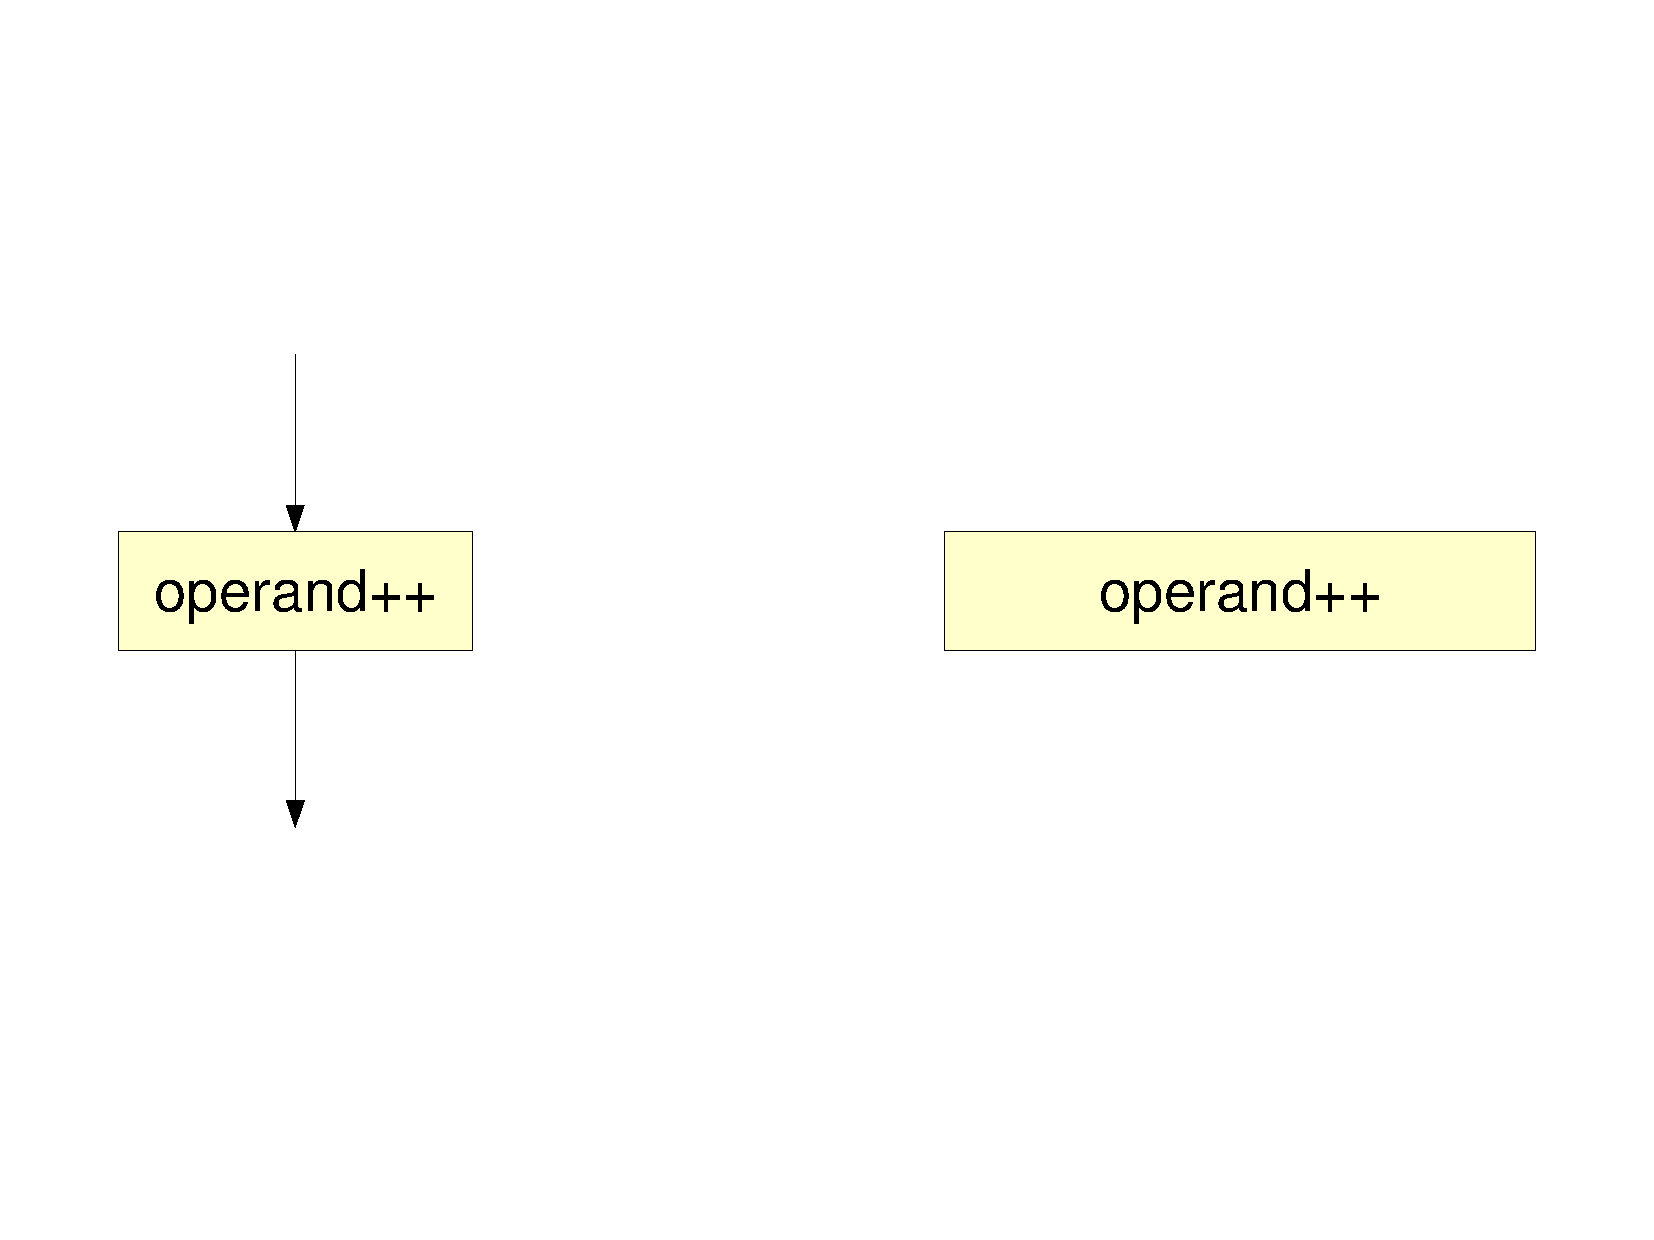
\includegraphics[scale=0.3,angle=-90]{graphic/statement.pdf}
        \caption{Statement as Program Flow Chart and Structure Chart}
        \label{statement_figure}
    \end{center}
\end{figure}

A \emph{Variable} is a placeholder for an abstracted \emph{Data Value}. It
occupies space in memory which is why this space has to be reserved before it
can be used. The reservation is called \emph{Allocation} or \emph{Declaration}
and it states the variable's \emph{Type} and an \emph{Identifier}. Commonly,
variables also get initialised through the \emph{Assignment} of an
\emph{Initial Value}. Here an example for declaration and initialisation
through assignment in \emph{C} code:

\begin{scriptsize}
    \begin{verbatim}
    type identifier = value;
    \end{verbatim}
\end{scriptsize}

Many statements which belong together can form a \emph{Block}, also called
\emph{Compound Statement}. Variables declared in a block are called its
\emph{Local Variables} and loose their validity outside that block. Blocks have
an opening and a closing symbol. Following once more an example in \emph{C}
programming language source code, showing a block with two statements:

\begin{scriptsize}
    \begin{verbatim}
    {
        statement1;
        statement2;
    }
    \end{verbatim}
\end{scriptsize}
